\section*{Introduction}

%NumPy is the fundamental array computation library for the Python
%ecosystem \cite{dubois2007guest,oliphant2007python,millman2011python,perez2011python}.
With its first stable release in October 2006, NumPy unified
the scientific Python community and now underpins almost every library
that does numerical computation, including SciPy\cite{virtanen2019scipy},
pandas\cite{mckinney-proc-scipy-2010}, scikit-learn\cite{pedregosa2011scikit},
and scikit-image\cite{vanderwalt2014scikit}.
Not surprisingly, many important scientific research projects and
results crucially rely on NumPy.
It plays an essential role in many research analysis pipelines in
fields as diverse as physics, biology, astronomy, neuroscience,
material science, engineering, and chemistry.
% w/ citations
In particular, NumPy played a fundamental role in discovering
gravitational waves\cite{pycbc} and the first imaging of a black
hole\cite{eht-imaging}, and lets us explore our
universe\cite{jenness2018lsst}.

%[LIGO, EHT, Higgs-Boson pipeline at CERN—double check this carefully,
%  may be root, ice cube experiment, https://arxiv.org/abs/1507.03989
%  IDL is now below Python, Pangeo <-> xarray, Earthcube,
%  https://ai.jpl.nasa.gov/public/documents/papers/hackett\_spaceops2018\_block.pdf,
%  Kepler, Mars rovers, SKA in South Africa, yt, astropy, seismo-live,
%  icesat2 \& icepyx, The Materials Project at LBNL https://github.com/materialsproject]

NumPy consists of the \code{ndarray}-object along with utility functions that
operate on it.
Because of its inherent simplicity—being a pointer to memory with some
associated meta-data about shape, data-type, and so forth—the NumPy array is
the {\it de facto} exchange format for array data in Python.
The library has such widespread adoption that not only the array object but also its
{\it Application Programming Interface} (API) has become ubiquitous as
a language for tensor computation---witnessed by its use in popular
deep learning libraries such as PyTorch\cite{pytorch}.

\subsection*{History}

Before NumPy, two different Python array packages—Numeric and NumArray—existed.
The first began in the mid-90s and was developed by Jim Fulton, Jim Hugunin,
Paul Dubois, Konrad Hinsen, Travis Oliphant, and others, and was aimed at fast
manipulation of many small arrays.
By the beginning of the millennium, several libraries built on top of Numeric 
to provide fundamental scientific routines were combined into SciPy.
Due to the poor performance of Numeric on large data sets, NumArray was
developed at the Space Telescope Science Institute (STScI) to handle
large astronomical images such as those produced by the Hubble Space Telescope.
However, while initially considered the successor to Numeric, NumArray was no longer
performant on multiple small arrays.
This divide posed a challenge for SciPy as it wasn't clear how to support
both libraries.
Working with the NumArray and SciPy communities, the then maintainer of Numeric,
Travis Oliphant, embarked upon a major rewrite that aimed to be a ``best of both
worlds'' unification of Numeric and NumArray. This merger resulted in NumPy.

The creation of NumPy spurred renewed development in both SciPy and the larger
scientific Python ecosystem and heralded the current era of wide-spread use of
Python for scientific computing.
To coordinate work as a global community, to ensure accuracy of computed
results, and to allow modification without breakage, the NumPy (and SciPy) teams
pioneered best software engineering practices in the scientific Python
community\cite{millman2014developing}.
For example, NumPy early on adopted distributed revision control, unit testing,
continuous integration, code review, and executable documentation.
It also developed a standard for ``docstrings''—text describing each NumPy function.
This quickly became a documentation standard for the larger scientific Python community. 

Travis Oliphant eventually stepped back from leading NumPy to found a
company and to start new projects including Numba---an accelerated Python
compiler that could vastly accelerate NumPy expressions.  Development
of NumPy continued by a core group that informally operated by
consensus.

% While the scientific Python community grew and new challenges arose, 

%By 2009, the project had entered a
%period of uncoordinated, opportunistic development, and was
%increasingly weighed down by technical debt that had accrued since the
%days of Numeric.

\subsection*{Funding}

For many years, NumPy had no dedicated funding, and development time
was mostly contributed freely by students and researchers in their
spare time.  In-person meetings were sponsored off of individual's
research grants, and while industry sponsored contributions were made,
notably those by Mark Wiebe when he was sponsored by Travis Oliphant
at Continuum Analytics, the package's rapid adoption in scientific
computing took place without external investment.

% BIDS -- UCB
% https://www.moore.org/grant-detail?grantId=GBMF5447
% $645,020 in 2016
% https://sloan.org/grant-detail/8222
% $659,359 in 2017
% https://bids.berkeley.edu/news/bids-receives-sloan-foundation-grant-contribute-numpy-development
In 2017, NumPy received its first large grants totaling 1.3M USD from the
Gordon \& Betty Moore and the Alfred P. Sloan foundations.
Stéfan van der Walt is the PI and manages four programmers working on the project.
These two grants focus on addressing the technical debt accrued over the years and
on setting in place standards and architecture to encourage more sustainable development.
% http://doi.org/10.5281/zenodo.3585761
% http://doi.org/10.5281/zenodo.3585767

% CZI -- NumFOCUS/QuanSight
% https://chanzuckerberg.com/eoss/proposals/strengthening-numpys-foundations-growing-beyond-code/
% NumPy and OpenBLAS received $195,000 in 2019
% https://labs.quansight.org/blog/2019/11/numpy-openblas-CZI-grant/
NumPy received another grant for \$195,000 from the Chan Zuckerberg
Initiative at the end of 2019 with Ralf Gommers as the PI.
This grant, building on the technical work supported by the previous
grant, will focus on better serving NumPy's large number of beginning
to intermediate level users and on growing the community of NumPy
contributors.
It will also provide support to OpenBLAS, on which NumPy depends for
accelerated linear algebra.

Finally, the project receives around 10K USD annually from Tidelift, which is
typically used to fund documentation writers and website developers.

\subsection*{Current status}

% (maturity, users)

As the NumPy release manager in 2007, Jarrod Millman, adopted the notion
of enhancement proposals---used infrequently and informally until 2017 when,
to facilitate work expected from funded development, he formalized the
NumPy Enhancement Proposal (NEP) process.  NEPs are modeled after
Python Enhancement Proposals (PEPs) for ``proposing major new
features, for collecting community input on an issue, and for
documenting the design decisions that have gone into
Python''\footnote{\url{https://numpy.org/neps/nep-0000.html}}.
Since then there have been 19 proposed NEPS---6 have been implemented,
4 have been accepted and are being implemented, 4 are under
consideration, 3 have been deferred or superseded, and 2 have been rejected
or withdrawn.

The first activities organized for the new grant were a NEP development
sprint, a weekly community call, and a meeting to write a draft roadmap.

Since the roadmap was meant to represent community consensus on future
development, it was presented for comment at the annual SciPy
conference during a so-called ``Birds of a Feather'' session, attended
by more than 100 people.  One additional meeting was held to discuss
specific enhancements, such as the development of a new data-type
system.  The final roadmap was vetted by the community via online
discussion before being accepted.

Weekly community calls alternate between triage and
higher level discussion.  The calls not only involve developers from
the community, but provide a venue for vendors and other external
groups to provide input.  For example, after Intel produced a forked
version of NumPy, one of their developers joined a call to discuss
community concerns.

NumPy plays a central role in building and standardizing much of the scientific
Python community infrastructure.
The docstring standard mentioned in the history section is now widely adopted.
We are also now using the NEP system as a way to help coordinate the larger
scientific Python community.
% https://numpy.org/neps/nep-0029-deprecation_policy.html
For example, in NEP 29, we recommend, along with leaders from various other
projects, that all projects across the Scientific Python ecosystem adopt a
common ``time window-based'' policy for support of Python and NumPy versions.
This standard will simplify downstream project and release planning.

% https://numpy.org/neps/scope.html
% https://numpy.org/neps/roadmap.html

%We showed that NumPy is actively developed according to a community
%vetted plan that integrates formal enhancement proposals.  Next, we
%give a more in-depth overview of the team developing NumPy, their
%activities, as well as the governance and community structures that
%guide the collaboration.

\section*{Project organization and community}

NumPy is currently maintained by a group of 23 contributors with commit rights
to the NumPy code base. Out of these, 17 maintainers were active in
2019, 4 of whom were paid to work on the project full-time.
Additionally, there are a few long term developers who contributed and maintain
specific parts of NumPy, but are not officially maintainers.
At a release cycle of about every half year, the five recent releases in the years
2018 and 2019 have averaged about 450~pull requests~(PRs) each,\footnote{
    Note that before mid 2011, NumPy development did not happen on \url{github.com}.
    All data provided here is based on the development which happened through GitHub
    pull requests. In some cases contributions by maintainers may not be categorized as such.}
% Since 1.14.0 (based on changelog): 381 + 438 + 490 + 531 + 402; last is preliminary
with each release attracting more than a hundred new contributors.

\begin{figure}
    \centering
    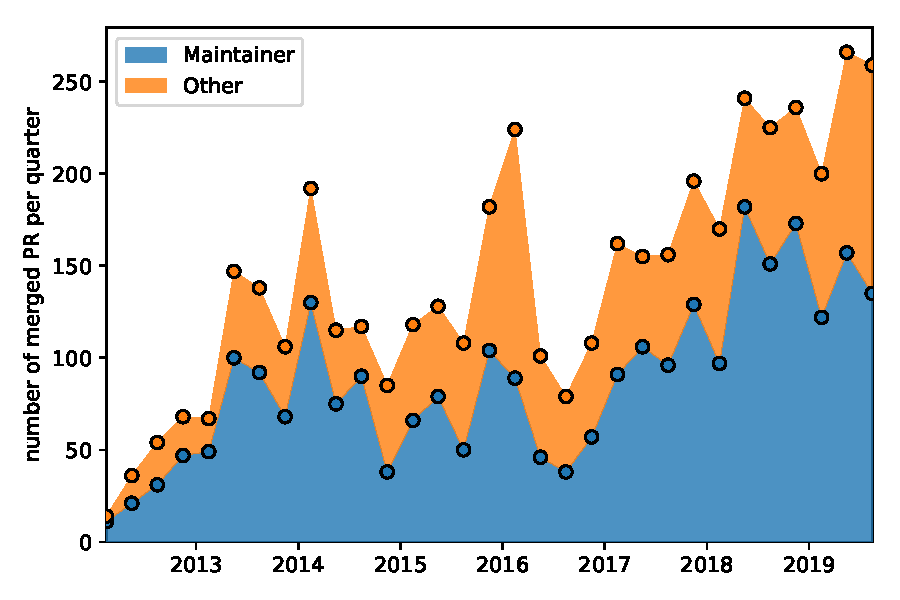
\includegraphics[width=0.5\textwidth]{scripts/PRs-using-CURRENT_MAINTAINERS.pdf}
    \caption{Number of pull requests merged into the NumPy master branch for each
        quarter since 2012. The total number of PRs is indicated with the
        lower blue area showing the portion contributed by current or previous
        maintainers.}\label{fig:prs-over-time}
\end{figure}

% -- The paragraphs above and below can be tightened up a bit still --

The stacked plot in Figure~\ref{fig:prs-over-time} shows the number of
PRs merged into the NumPy master branch.
In this plot PRs opened by current and old maintainers are indicated.
Although the number of PRs being merged fluctuates,
the plot indicates an increased number of contributions over the past
years.
Over the course of its history, NumPy has attracted PRs by 823 contributors.
However, its development relies heavily on a relatively small number
of active maintainers, who share more than half of the contributions among
themselves.

% https://mail.python.org/pipermail/numpy-discussion/2015-October/073849.html
% https://github.com/numpy/numpy/pull/6352
To formalize its unwritten development policy,
NumPy adopted an official Governance Document on October~5,
2015\cite{NumPyProjectGovernance}.
Project decisions are usually made by consensus of interested contributors.
This means for many thing everyone is entrusted with veto power.
A Steering Council, currently composed of 12~members, facilitates this
process and oversees daily development of the project by contributing code
and reviewing contributions from the community.

% https://mail.python.org/pipermail/numpy-discussion/2018-July/078476.html
% https://github.com/numpy/numpy/pull/11865
NumPy's official Code of Conduct was approved on September~1, 2018\cite{NumPyCodeofConduct}.
In brief, we strive to:
\emph{be open};
\emph{be empathetic, welcoming, friendly, and patient};
\emph{be collaborative};
\emph{be inquisitive}; and
\emph{be careful in the words that we choose}.
The Code of Conduct also specifies how breaches can be reported and outlines
the process for responding to such reports.

\section*{Library organization}

The NumPy library consists of core functionality (e.g., the NumPy array data structure),
functions for manipulating arrays and doing scientific computation, and infrastructure
libraries.

\subsection*{Core}

The \code{ndarray} data structure stores regularly spaced elements of a single
data type in a contiguous block of memory; along with meta-data such as shape,
it allows for the efficient representation of $n$-dimensional arrays.
More details about the data structure are given in ``The NumPy array:
a structure for efficient numerical computation.''\cite{vanderwalt2011numpy}.

\begin{figure}
  \centering
  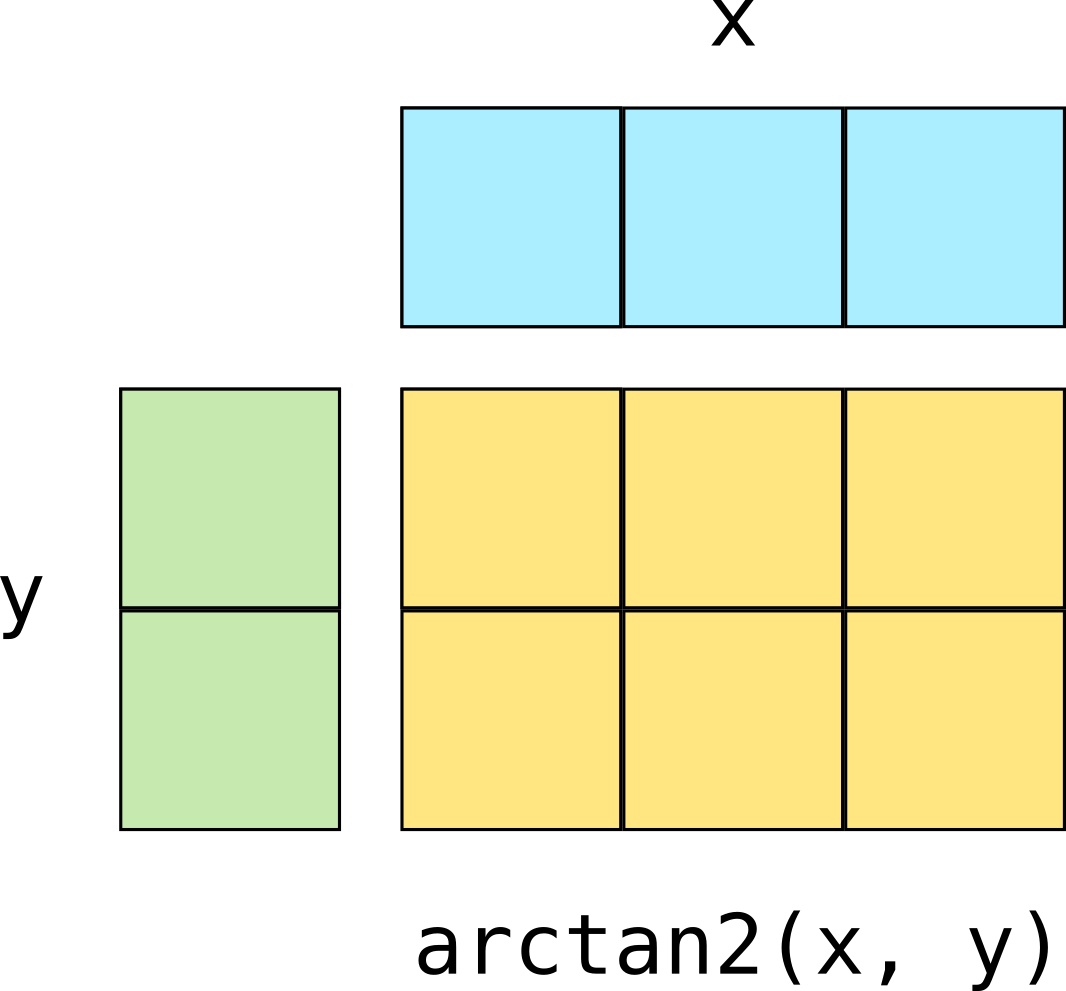
\includegraphics[width=0.25\textwidth]{static/broadcasting}
  \caption{
    Broadcasting a $1 \times 3$ array against a $2 \times 1$ array
    yields a $2 \times 3$ result.
  }
  \label{fig:broadcasting}
\end{figure}

The \emph{universal functions} (or \emph{ufuncs})
are functions written in C that implement efficient looping over
NumPy arrays. An important feature of ufuncs is the built-in
implementation of \emph{broadcasting}.  For example, the function
\code{arctan2(x, y)} is a ufunc that accepts two arguments and computes
$\tan^{-1}(y/x)$.  The ufunc loops over the dimensions of the inputs
in such a way that if, say, \code{x} is a 1-d array with length 3, and
\code{y} is a 2-d array with shape $2 \times 1$, the output will be
an array with shape $2 \times 3$ (see Figure~\ref{fig:broadcasting}).  The ufunc machinery takes care
of calling the function with all the appropriate combinations of
input array elements to compute the output array.
The elementary arithmetic operations of addition, multiplication, etc.,
are implemented as ufuncs, so broadcasting applies even in expressions
such as \code{x + y * z}.

\subsection*{Computing libraries}

NumPy provides a large collection of functions for array manipulation
including functions for: creating, reshaping, concatenating, and padding arrays;
searching, sorting and counting data
in arrays; computing elementary statistics, such as the mean, median,
variance, and standard deviation; file I/O; and more.
It also provides extensive support for generating pseudorandom numbers
as well as an assortment of probability distributions.
For historical reasons, NumPy also includes basic functionality for
linear algebra, fast Fourier transforms and windowing,
and polynomial fitting.
We will continue supporting these, but we will not expand beyond them.

\subsection*{Infrastructure libraries}

NumPy also provides basic infrastructure for other packages in the scientific
Python ecosystem.
The \code{numpy.testing} subpackage provides functions such as
\code{assert\_allclose(actual, desired)} that may be used in unit
test suites for code that uses NumPy arrays.
The \code{numpy.distutils} subpackage provides build support for C++, Fortran,
BLAS/LAPACK, and other relevant libraries for scientific computing.
The program \code{f2py} is a tool for
building NumPy-aware Python wrappers of Fortran functions.
NumPy itself does not use any Fortran code;  F2PY is part of NumPy
for historical reasons.

\section*{Recent technical improvements}

The NumPy codebase has been actively developed for over two decades (first as
Numeric and NumArray).
Given the complexity of the codebase and the massive number of projects depending
on it, large changes require careful planning and substantial work.
Moreover, with the now prevalent need for distributed computing and the
emergence of specialized hardware such as GPUs, many new usecases have
arisen, which NumPy was not originally designed for.
With the recent infusion of funding and the newly formalized NEP process in
place we have been able to tackle a number of important large scale changes.
We highlight two of those below, as well as changes made to our testing
infrastructure to support hardware platforms used in large scale computing.

\subsection*{The Array Function Protocol}

A vast number of projects are built on NumPy;
these projects are consumers of the NumPy API.
%The central position of NumPy takes within the numerical and scientific
%Python ecosystem means that a vast number of projects are built on it.
%These projects are consumers of the NumPy API.
Over the last several years, a growing number of projects are providers of
a \emph{NumPy-like API} and array objects targeting audiences with specialized
needs beyond NumPy's capabilities.
For example, the NumPy API is implemented by several popular tensor computation
libraries including CuPy\footnote{\url{https://cupy.chainer.org/}},
Jax\footnote{\url{https://jax.readthedocs.io/en/latest/jax.numpy.html}},
PyTorch\footnote{\url{https://pytorch.org/tutorials/beginner/blitz/tensor\_tutorial.html}}, and
and Apache MXNet\footnote{\url{https://mxnet.incubator.apache.org/api/python/docs/api/ndarray/index.html}}.
It is also implemented in packages that support sparse arrays
such as \code{scipy.sparse} and \code{pydata.sparse}.
Another notable example is Dask, a library for parallel computing in
Python.  Dask adopts the NumPy API and therefore presents a familiar
interface to existing NumPy users, while adding powerful abilities to
parallelize and distribute tasks.

The multitude of specialized projects creates the difficulty that consumers
of these NumPy-like APIs write code specific to a single project and do not support
all of the above array providers.
This is a burden for users relying on the specialized array-like, since
a tool they need may not work for them.
It also creates new challenges for end-users who need to transition
from NumPy to a more specialized array.
The growing multitude of specialized projects with NumPy-like APIs threatened
to again fracture the scientific Python community.

To address these issues NumPy has the goal of providing the fundamental
API for \emph{interoperability} between the various NumPy-like APIs.
An earlier step in this direction was the implementation of the
\code{\_\_array\_ufunc\_\_} protocol in NumPy 1.13, which enabled interoperability
for most mathematical functions.\cite{NEP13}
In 2019 this was expanded more generally with the inclusion of the
\code{\_\_array\_function\_\_} protocol into NumPy~1.17.
These two protocols allows providers of array-like APIs to be interoperable
with the NumPy API: their arrays work correctly with almost all NumPy functions.\cite{NEP18}
For the users relying on specialized array projects it means that even though
much code is written specifically for NumPy arrays and uses the NumPy API as
\code{import numpy as np}, it can nevertheless work for them.  For
example, here is how a CuPy GPU array can be passed through NumPy for
processing, with all operations being dispatched back to CuPy:

\begin{lstlisting}
import numpy as np
import cupy as cp

x_gpu = cp.array([1, 2, 3])
y = np.sum(x_gpu)  # This works, and returns a GPU array
\end{lstlisting}


Similarly, user defined functions composed using NumPy can now be
applied to, e.g., multi-node distributed Dask arrays:

\begin{lstlisting}
import numpy as np
import dask.array as da


def f(x):
    """Function using NumPy API calls"""
    y = np.tensordot(x, x.T)
    return np.mean(np.log(y + 1))


x_local = np.random.random([10000, 10000])  # random local array
x_distr = da.random.random([10000, 10000])  # random distributed array

f(x_local)  # returns a NumPy array
f(x_distr)  # works, returns a Dask array
\end{lstlisting}

\subsection*{Random}

%The random number generator library in NumPy provides several alternative
%\emph{bit stream generators} that provide the core function of generating
%random integers.
%A higher-level generator class that implements an assortment of
%probability distributions is provided. It includes the beta, gamma
%and Weibull distributions, the univariate and multivariate normal
%distributions, and more.

The NumPy random module provides pseudorandom numbers from a wide range of
distributions. In legacy versions of NumPy, simulated random values are produced
by a \code{RandomState} object that: handles seeding and state initialization;
wraps the core pseudorandom number generator based on a 32-bit implementation of
MT19937; interfaces with the underlying code that transforms random bits into
deviates from other distributions; and supplies a singleton instance exposed in
the root of the random module.

The \code{RandomState} object makes a compatibility guarantee so that a fixed
seed and sequence of function calls produce the same set of values. This
guarantee has slowed progress since improving the underlying code requires
extending the API with additional keyword arguments. This guarantee continues to
apply to \code{RandomState}. 

% Mention explicitly the NEPs involved

NumPy 1.17 introduced a new API for generating random numbers that use a more
flexible structure that can be extended by libraries or end-users. The new API
is built using components that separate the steps required to generate random
variates. Pseudorandom bits are generated by a bit generator. These bits are
then transformed into variates from complex distributions by a generator.
Finally, seeding is handled by an object that produces sequences of high-quality
initial values.

Bit generators are simple classes that manage the state of an underlying
pseudorandom number generator. NumPy ships with four bit generators. The default
bit generator is a 64-bit implementation of the Permuted Congruential Generator
\cite{pcg64} (\code{PCG64}). The three other bit generators are a 64-bit version
of the Philox generator\cite{random123} (\code{Philox}), Chris Doty-Humphrey's
Small Fast Chaotic generator\cite{practrand} (\code{SFC64}), and the 32-bit
Mersenne Twister\cite{mt19937} (\code{MT19937}) which has been used in older
versions of NumPy.\footnote{The
\href{https://github.com/bashtage/randomgen}{randomgen project} supplies a wide
range of alternative bit generators such as a cryptographic counter-based
generators (\code{AESCtr}) and generators that expose hardware random number
generators (\code{RDRAND})\cite{randomgen}.} Bit generators export a capsule
containing pointers to functions that produce 64 bits, 32 bits, or a random
double. They also expose CFFI and ctypes interfaces to the same three functions.

The \code{Generator} consumes one of the bit generators and produces variates
from complicated distributions. Many improved methods for generating random
variates from common distributions were implemented, including the Ziggurat
method for normal, exponential and gamma variates\cite{ziggurat}, and Lemire's
method for bounded random integer generation\cite{lemire}. The \code{Generator}
is more similar to the legacy \code{RandomState}, and its API is substantially
the same. The key differences all relate to state management, which has been
delegated to the bit generator. The \code{Generator} does not make the same
stream guarantee as the \code{RandomState} object, and so variates may differ
across versions as improved generation algorithms are
introduced.\footnote{Despite the removal of the compatibility guarantee, simple
reproducibility across versions is encouraged, and minor changes that do not
produce meaningful performance gains or fix underlying bug are not generally
adopted.}

Finally, a \code{SeedSequence} is used to initialize a bit generator. The seed
sequence can be initialized with no arguments, in which case it reads entropy
from a system-dependent provider, or with a user-provided seed. The seed
sequence then transforms the initial set of entropy into a sequence of
high-quality pseudorandom integers, which can be used to initialize multiple bit
generators deterministically. A key design goal of a seed sequence was to be
splittable in the sense that a seed sequence can be used to produce child
sequences that are distinct from their parents or other ancestors. This
capability allows a seed sequence to be used in large distributed applications
where the number of workers required is not known. The sequences generated from
the same initial entropy and the same splits are fully deterministic to ensure
reproducibility.

The three components are combined to construct a complete random number
generator.

\begin{lstlisting}
from numpy.random import Generator, PCG64, SeedSequence

seq = SeedSequence(10304245474441179933310169597522947680)
pcg = PCG64(seq)
gen = Generator(pcg)
\end{lstlisting}

\noindent This approach retains access to the seed sequence which can then be
used to spawn additional generators.

\begin{lstlisting}
children = seq.spawn(2)
gen_0 = Generator(PCG64(children[0]))
gen_1 = Generator(PCG64(children[1]))
\end{lstlisting}

\noindent While this approach retains complete flexibility, the method
\code{np.random.default\_rng} can be used to instantiate a \code{Generator} when
reproducibility is not needed.

The final goal of the new API is to improve extensibility. \code{RandomState} is
a monolithic object that obscures all of the underlying state and functions. The
component architecture is one part of the extensibility improvements. The
underlying functions (written in C) which transform the output of a bit
generator to other distributions are available for use in CFFI. This allows the
same code to be run in both NumPy and dependent that can consume CFFI, e.g.,
Numba. Both the bit generators and the low-level functions can also be used in C
or Cython code.\footnote{As of 1.18.0, this scenario requires access to the
NumPy source. Alternative approaches that avoid this extra step are being
explored.} 

\subsection*{Testing on multiple architectures}

At the time of writing the two fastest supercomputers in the
world, Summit and Sierra, both have IBM POWER9 architectures
\cite{top500nov2019}. In late 2018, Astra, the first ARM-based
supercomputer to enter the TOP500 list, went into production\cite{
astra-wiki}. Furthermore, over 100 billion ARM processors have been
produced as of 2017\cite{arm-architecture}, making it the most 
widely used instruction set architecture in the world.

Clearly there are motivations for a large scientific computing
software library to support POWER and ARM architectures. We've extended
our continuous integration (CI) testing to include \texttt{ppc64le}
(POWER8 on Travis CI) and ARMv8 (on Shippable service). We also test
with the s390x architecture (IBM Z CPUs on Travis CI) so that we
can probe the behavior of our library on a big-endian machine.
This satisfies one of the major components of
improved CI testing laid out in a version of our roadmap
\cite{numpy-roadmap}---specifically, ``CI for more exotic
platforms."

PEP 599\cite{PEP599} lays out a plan for new Python binary wheel
distribution support, \texttt{manylinux2014}, that adds
support for a number of architectures supported by the CentOS
Alternative Architecture Special Interest Group, including
ARMv8, ppc64le, as well as s390x. We are thus well-positioned
for a future where provision of binaries on these architectures
will be expected for a library at the base of the ecosystem.


\section*{Discussion}

% 1st grant done, technical cleanup finished except dtypes
% 2nd grant starting, community growth and new user focus

Most of the technical work for the Moore and Sloan grant is now complete.
The main remaining item is an overhaul of the data type system, which
we are currently working on \href{https://github.com/numpy/numpy/pull/14422}{draft of DTypes NEP}].
The meaning of each element within a NumPy array is described by its
datatype (dtype). NumPy arrays can hold all common numerical
datatypes, strings, datetimes, and generic Python objects, each of
which is identified by a dtype.
%We are busy overhauling the datatype
%system to make it behave consistently and to simplify the creation of
%custom dtypes, both in C and in Python [XXX Cite the NEP here, instead
%of \href{https://github.com/numpy/numpy/pull/14422}{draft of DTypes NEP}].
While numerical dtypes make the foundation for most users,
there are a multitude of use cases which cannot prosper due to current
limitations, such as physical units\cite{astropy,Goldbaum2018,pint},
% pyadolc may be a bit too small a project, so may want to remove/replace with an other example.
geometrical objects\cite{pygeos}, and automatic
differentiation\cite{pyadolc}.
%Projects addressing these exist, each struggles with current
%limitations.  % TODO: I may need citations, we could link github issues.
The proposed overhaul of the datatype system will make it behave consistently and
to simplify the creation of custom dtypes, both in C and in Python

%% While it is currently possible to define custom dtypes within NumPy, many of the
%% use cases above cannot be solved using this system.
%% This is evidenced also by code within NumPy which would require changes
%% in many places to add such dtypes, even when adding them within NumPy itself.
%% The new implementation will be simpler and more cleanly implemented in
%% this regard.
%% Custom dtypes and the basic dtypes included within NumPy will be implemented
%% and behave identically as much as possible.
%% At the same time redesigning the API will make NumPy dtypes more flexible to grow
%% to future needs should they arise.

%% As a further step, to make dtypes more accessible and allow a faster adoption of
%% custom dtypes within the community, we plan to create a Python API to
%% define such custom dtypes.

Having made progress on addressing technical debt accrued over two decades of
development and modernizing the code to handle new use cases, the project
is ready to grow its community of contributors and to better address the needs
of an ever-growing number of new users.  This is the main focus of the
forthcoming CZI grant.

[... CZI grant ...]

[... welcome new users ...]

% technical focus
% improve various aspects of NumPy, including easier construction of custom data types (e.g., missing values, physical units, times & dates) and better integration with arrays customized for specialized domains (e.g., SciPy's sparse arrays, pandas' DataFrames, and xarray's labeled arrays). 
% technical work, and it increased the velocity of the projects by ~25-30%, and in addition it enabled integrating some larger changes, like the numpy.random redesign.


% \subsubsection*{Future Development}

% Dtypes

% outline plan for the CZI grant and an invitation to new contributors

%\subsection*{Website}
